\documentclass[a4paper,10pt]{article}
\usepackage[a4paper,margin=10mm]{geometry}
\usepackage{tikz}
\usepackage{helvet}
\renewcommand{\familydefault}{\sfdefault}
\pagestyle{empty}
\setlength{\parindent}{0pt}
\begin{document}

{\Large\bfseries ODOMETRY 90\textdegree{} TURN --- ANGLE REFERENCE SHEET}\par
\vspace{1mm}
{\small Print on A4 at 100\% scale (disable fit-to-page). Tape the sheet flat to the desk.
Place the robot centred on the cross, facing 0\textdegree{} (up). Press the button once.
After it stops, read the final heading where the robot's centreline crosses the arc.
Ticks are 5\textdegree; major labels every 30\textdegree.}\par
\vspace{2mm}

\begin{center}
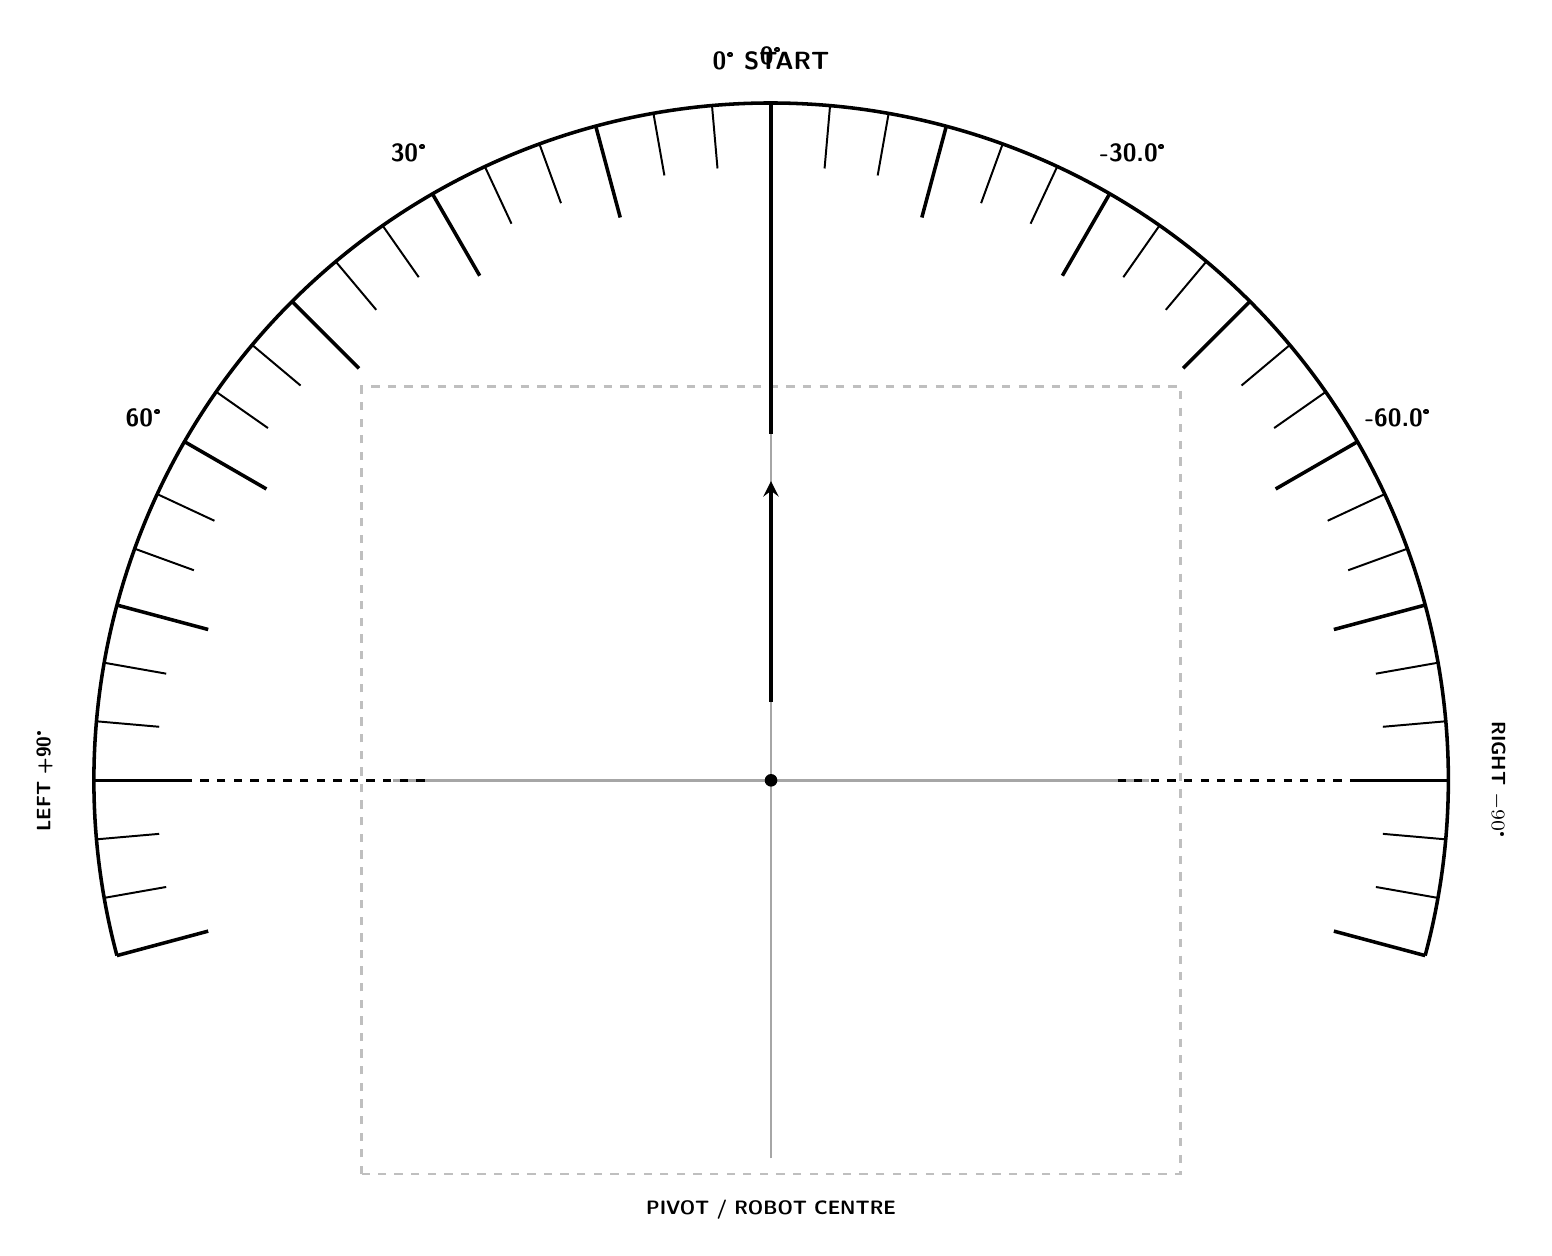
\begin{tikzpicture}[x=1mm,y=1mm]

  % Pivot and robot footprint (roughly 97 x 92 mm, front towards 0 deg/up)
  \coordinate (O) at (0,0);
  \draw[gray!50, dashed, line width=0.3mm] (-52,-50) rectangle (52,50);
  \draw[gray!70, line width=0.3mm] (0,-48) -- (0,48);
  \draw[gray!70, line width=0.3mm] (-48,0) -- (48,0);
  \fill[black] (O) circle (0.8);
  \node[font=\scriptsize\bfseries, below] at (0,-52) {PIVOT / ROBOT CENTRE};

  % Arc and ticks. Turn angle phi: 0 deg = forward, +left, -right.
  \draw[line width=0.45mm] (-15:86) arc (-15:195:86);
  \foreach \p in {-105,-100,...,105} {
    \pgfmathsetmacro{\ang}{90+\p}
    \draw[line width=0.25mm] (\ang:78) -- (\ang:86);
  }
  % Major ticks every 15 deg, labels every 30 deg
  \foreach \p in {-105,-90,-75,-60,-45,-30,-15,0,15,30,45,60,75,90,105} {
    \pgfmathsetmacro{\ang}{90+\p}
    \draw[line width=0.45mm] (\ang:74) -- (\ang:86);
  }
  \foreach \p in {-60,-30,0,30,60} {
    \pgfmathsetmacro{\ang}{90+\p}
    \pgfmathsetmacro{\lab}{\p}
    \node[font=\small\bfseries, fill=white, inner sep=0.5mm] at (\ang:92) {\lab\textdegree};
  }

  % Reference rays
  \draw[line width=0.6mm] (0,44) -- (0,86);
  \draw[line width=0.35mm, dashed] (90+90:44) -- (90+90:86);
  \draw[line width=0.35mm, dashed] (90-90:44) -- (90-90:86);

  \node[font=\small\bfseries, anchor=south] at (0,89) {0\textdegree{} START};
  \node[font=\scriptsize\bfseries, rotate=90, anchor=south] at (90+90:90) {LEFT +90\textdegree};
  \node[font=\scriptsize\bfseries, rotate=-90, anchor=south] at (90-90:90) {RIGHT $-90$\textdegree};

  % Arrow showing robot forward direction at the start
  \draw[line width=0.5mm, ->, >=stealth] (0,10) -- (0,38);

\end{tikzpicture}
\end{center}

\vspace{1mm}
{\footnotesize\bfseries Notes.}
{\footnotesize
Read the angle at the end of the robot's centreline, using the ticks outside the robot body.
The expected 90\textdegree{} references are the two dashed rays. A reading of, for example,
94\textdegree{} means the robot physically over-rotated by 4\textdegree{} relative to the intended junction turn.
The sheet does not guide the robot; it is only an independent visual reference for the final heading.}

\end{document}
